\documentclass[sigplan,screen]{acmart}
\let\Bbbk\relax

\renewcommand\footnotetextcopyrightpermission[1]{}
\pagestyle{plain}

\usepackage{xr}
\usepackage{amsmath,amssymb}
\usepackage{proof}
\usepackage{listings}
\usepackage{tikz}
\usetikzlibrary{shapes.geometric, shapes.multipart, arrows.meta, positioning, calc}

\tikzstyle{startstop} = [rectangle, rounded corners, minimum width=3cm, minimum height=1cm,text centered, draw=black, fill=gray!20]
\tikzstyle{process} = [rectangle, minimum width=3cm, minimum height=1cm, text centered, draw=black, fill=blue!10]
\tikzstyle{decision} = [diamond, aspect=2, draw=black, fill=orange!20, text centered]
\tikzstyle{arrow} = [thick, ->, >=stealth]

\overfullrule = 1cm

\title{Supplementary Materials for: Merkle Tree-Based Inheritance in Decentralized Module Systems}

\begin{CCSXML}
<ccs2012>
   <concept>
       <concept_id>10011007.10011006.10011008</concept_id>
       <concept_desc>Software and its engineering~Software design techniques</concept_desc>
       <concept_significance>500</concept_significance>
   </concept>
   <concept>
       <concept_id>10002944.10011123.10011131</concept_id>
       <concept_desc>General and reference~Evaluation</concept_desc>
       <concept_significance>300</concept_significance>
   </concept>
</ccs2012>
\end{CCSXML}

\ccsdesc[500]{Software and its engineering~Software design techniques}
\ccsdesc[300]{General and reference~Evaluation}

\keywords{Merkle trees, decentralized systems, module inheritance, software design, evaluation}

\begin{document}

\maketitle

\appendix
\section{Formal Properties of Finalization}
\label{appendix:formal-properties}

I now formally state and prove the core semantic properties of my finalization model: \textbf{Determinism}, \textbf{Injectivity}, and \textbf{Soundness}.

\subsection{Determinism}
\label{appendix:determinism}

\begin{theorem}[Determinism of Finalization]
\label{thm:determinism}
For all inputs $(C, T, A, \{r_1, \ldots, r_n\})$, finalization always produces a unique result. That is:
\[
\mathcal{F}(C, T, A, \{r_1, \ldots, r_n\}) = h_M
\]
is a total and deterministic function.
\end{theorem}

\begin{proof}
Each step of $\mathcal{F}$ consists of deterministic subcomputations:
\begin{itemize}
    \item $\mathcal{R}$ resolves symbolic names to hashes via a fixed registry map.
    \item Ancestry $A(M)$ is constructed by recursive union over parents, deterministically ordered.
    \item The Merkle root $H_{\text{merkle}}(P)$ is computed from a lexicographically sorted list, ensuring unique tree layout.
    \item Content hashing $h_C = H(C)$ and final ID computation $h_M = H(h_C || T || A || H_{\text{merkle}}(P))$ are purely functional.
\end{itemize}
All operations are total and deterministic, thus $\mathcal{F}$ is deterministic.
\end{proof}
\subsection{Injectivity}
\label{appendix:injectivity}

\begin{theorem}[Injectivity of Finalization]
\label{thm:injectivity}
If \\$\mathcal{F}(C_1, T_1, A_1, P_1) = \mathcal{F}(C_2, T_2, A_2, P_2)$, then:
\[
(C_1, T_1, A_1, P_1) = (C_2, T_2, A_2, P_2)
\]
\end{theorem}

\begin{proof}
Assume $h_1 = \mathcal{F}(C_1, T_1, A_1, P_1)$ and \\$h_2 = \mathcal{F}(C_2, T_2, A_2, P_2)$ and $h_1 = h_2$.

Then:
\[
H(h_{C_1} || T_1 || A_1 || H_{\text{merkle}}(P_1)) = H(h_{C_2} || T_2 || A_2 || H_{\text{merkle}}(P_2))
\]

Since $H$ is a cryptographic hash function with collision resistance, the input tuples must be byte-for-byte identical:
\[
(h_{C_1}, T_1, A_1, H_{\text{merkle}}(P_1)) = (h_{C_2}, T_2, A_2, H_{\text{merkle}}(P_2))
\]

Thus $C_1 = C_2$, $T_1 = T_2$, $A_1 = A_2$, and $P_1$ and $P_2$ have identical Merkle roots. Because the Merkle tree is built over a sorted list of finalized IDs, equality of Merkle roots implies identical parent sets. Hence, inputs are equal.
\end{proof}

\subsection{Monotonicity}
\label{appendix:monotonicity}

\begin{theorem}[Monotonicity of Finalization]
\label{thm:monotonicity}
Let $M_1 \sqsubset M_2$ denote that $M_2$ is a refinement of $M_1$ (i.e., $C_1 \subseteq C_2$ and $T_1 = T_2$, $A_1 = A_2$, $P_1 = P_2$). Then:
\[
M_1 \sqsubset M_2 \Rightarrow H(M_1) \neq H(M_2)
\]
but
\[
\quad \text{ResolutionTable}(M_1) \subseteq \text{ResolutionTable}(M_2)
\]
\end{theorem}

\subsection{Termination}
\label{appendix:termination}

\begin{theorem}[Termination of Finalization]
\label{thm:termination}
Finalization always terminates on well-formed input:
\[
\forall M.\ \text{acyclic}(A(M)) \Rightarrow \exists h_M.\ \mathcal{F}(C, T, A, P) \Downarrow h_M
\]
\end{theorem}

\begin{proof}
Finalization proceeds in the following bounded steps:
\begin{enumerate}
    \item \textbf{Symbolic resolution} is finite over a finite set of references $\{r_1, \dots, r_n\}$.
    \item \textbf{Ancestry expansion} is a recursive set-union traversal over the parent graph. Since $A(M)$ is acyclic and finite (each module has a finite number of parents), the recursion always terminates.
    \item \textbf{Merkle tree construction} uses a lexicographically sorted list of finalized parent hashes, which is a finite and terminating computation.
    \item \textbf{Hashing} operations are total and constant-time.
\end{enumerate}
Since all substeps are terminating, $\mathcal{F}$ terminates on any well-formed acyclic input.
\end{proof}

\begin{proof}
The final hash includes $H(C)$ as a component. If $C_1 \subset C_2$, then $H(C_1) \neq H(C_2)$ with overwhelming probability (by hash injectivity). Therefore, $H(M_1) \neq H(M_2)$.

For resolution, since $M_2$ adds only new declarations and does not remove or shadow any from $M_1$, the computed resolution table extends that of $M_1$. Resolution proceeds left-to-right along a fixed linearization of $A$, so new entries in $C_2$ appear earlier or extend the resolution domain, preserving all bindings from $M_1$.
\end{proof}

\begin{corollary}[Stability under Extension]
\label{cor:stability-extension}
Finalizing a module $M$ multiple times with extended content (but fixed ancestry and types) produces distinct IDs, but earlier bindings remain valid:
\[
\text{If } M \sqsubset M', \text{ then } R_M \subseteq R_{M'}
\]
\end{corollary}

\subsection{Soundness}
\label{appendix:soundness}

\begin{theorem}[Symbol Resolution Soundness]
\label{thm:soundness}
Let $M$ be a finalized module with resolution table $R_M$ computed at finalization time. Then for every $s \in \text{dom}(R_M)$:
\[
M \vdash s \Downarrow d \leadsto \pi \quad\text{and}\quad \Gamma \vdash d : \tau
\]
and if $s$ overrides a parent symbol $s'$, then:
\[
\Gamma(d) <: \Gamma(s')
\]
\end{theorem}

\begin{proof}
Resolution uses a fixed order over $A(M)$ defined by Merkle ordering. For each $s$, the first provider $M_i$ is selected uniquely. By determinism of this ordering, $M_i$ is unique, and so is $d$.

Type soundness follows from override checks during finalization. For any override, finalization verifies that the overriding type $\tau'$ is a subtype of the overridden type $\tau$, satisfying $\tau' <: \tau$. Since typing is preserved under subtyping, all symbol uses remain valid.
\end{proof}

\subsection{Corollary: Functional Resolution}
\label{appendix:corollary-functional}

\begin{corollary}
Symbol resolution is a partial function:
\[
R_M : \text{name} \rightharpoonup (M_i, s_j)
\]
and if $M \vdash s \Downarrow d_1$ and $M \vdash s \Downarrow d_2$, then $d_1 = d_2$.
\end{corollary}

\begin{proof}
Immediate from the uniqueness property of Merkle ordering and Theorem~\ref{thm:determinism}.
\end{proof}

\section{Formal Resolution and Override Rules}

\subsection{Symbol Resolution and Override Traces}
\label{sec:resolution-traces}

Tangl resolves symbols using a breadth-first search (BFS) traversal over the module inheritance graph, starting from the child and proceeding to its ancestors. This design guarantees predictable symbol resolution across arbitrarily deep module graphs and avoids the ambiguity of linear inheritance. 

\paragraph{Resolution Semantics}
\begin{itemize}
  \item Resolution is performed using a child-first breadth-first search.
  \item Symbols are identified by their \texttt{name} and \texttt{scope}.
  \item If multiple symbols with the same name and scope appear during traversal, only the first encountered (i.e., closest to the child) is retained.
  \item If a symbol is aliased during import, its resolution respects the alias rather than the original name.
  \item Only the final resolved set of symbols is stored in the module's public symbol table.
\end{itemize}

\paragraph{Overrides and Traces}
\begin{itemize}
  \item Overridden symbols are not discarded: they are tracked via metadata linking each symbol to its parent module and override history.
  \item A future extension will introduce a dedicated query API for retrieving override chains.
  \item Currently, override traces require manual traversal of the parent chain using the symbol metadata.
\end{itemize}

\paragraph{Error Behavior}
Resolution failures result in descriptive error messages and occur in the following cases:
\begin{itemize}
  \item A symbol is referenced that does not exist in any reachable parent.
  \item Two aliased symbols with the same alias name are imported.
  \item A malformed import produces an invalid scope or alias.
\end{itemize}

\paragraph{Cyclic Dependencies}
Cyclic inheritance is structurally forbidden in the module graph; therefore, resolution is guaranteed to terminate.

\subsection{Resolution Inference Rules}

I define a judgment $\Gamma \vdash M \Downarrow \Sigma$ meaning that under module context $\Gamma$, the module $M$ resolves to symbol table $\Sigma$.

\textbf{[Resolve-Empty]}
\[
\frac{~}{\Gamma \vdash M[\ ] \Downarrow \{\}}
\]

\textbf{[Resolve-Self]}
\[
\frac{\text{sym} \in \text{Symbols}(M)}{\Gamma \vdash M[\texttt{sym}] \Downarrow \{\texttt{name} \mapsto \texttt{sym}\}}
\]

\textbf{[Resolve-Parent]}
\[
\frac{
  \Gamma \vdash P \Downarrow \Sigma \quad 
  \texttt{name} \notin \text{dom}(\text{Symbols}(M))
}{
  \Gamma \vdash M \Downarrow \Sigma \cup \text{Symbols}(M)
}
\]

\textbf{[Resolve-Alias]}
\[
\frac{
  \Gamma \vdash P \Downarrow \Sigma \quad 
  \Sigma(\texttt{name}) = \texttt{sym}
}{
  \Gamma \vdash \texttt{alias name} \mapsto \texttt{sym}
}
\]

\textbf{[Resolve-Conflict]}
\[
\frac{
  \Gamma \vdash P_1 \Downarrow \Sigma_1 \quad
  \Gamma \vdash P_2 \Downarrow \Sigma_2 \quad
  \texttt{name} \in \text{dom}(\Sigma_1) \cap \text{dom}(\Sigma_2)
}{
  \Gamma \vdash \text{error: conflicting symbol definitions}
}
\]

\subsection{Override Trace}

Given a resolved symbol $\texttt{sym}$ in module $M$, I define its override trace as the sequence:
\[
\texttt{trace(sym)} = [\texttt{sym}_0, \texttt{sym}_1, \dots, \texttt{sym}_n]
\]
where $\texttt{sym}_0$ is defined in $M$ and each $\texttt{sym}_{i+1}$ is the symbol it overrides in $M$'s parent graph.

Currently, this trace must be computed manually by walking the parent chain; future work includes exposing this trace via a query API.

\subsection{Symbol Metadata and Override Trace (Formal Version)}

Each symbol $s$ carries associated metadata recording:
\begin{itemize}
    \item Its \emph{origin} module $M_s$ where it was initially defined.
    \item (Optional) A reference $\mathsf{parent}(s)$ to the immediate symbol it overrides, if any.
\end{itemize}

\paragraph{Override Relation}
I define the \emph{override relation} $\prec$ between symbols:
\[
s' \prec s \quad \text{iff} \quad \mathsf{parent}(s) = s'
\]
That is, $s$ overrides $s'$ if $s'$ is the parent of $s$ in metadata.

\paragraph{Override Chain (Trace)}
The \emph{override chain} (or trace) from a symbol $s$ is the sequence $s_0, s_1, s_2, \dots$ where:
\[
s_0 = s
\]
\[
\forall i \geq 0.\ \mathsf{parent}(s_i) = s_{i+1}
\]
and $\mathsf{parent}(s_n) = \varnothing$ for some $n$, terminating the chain.

\paragraph{Inference Rules for Traversal}
\[
\infer[\textsc{Trace-Term}] {s \Downarrow [\ ]} {
    \mathsf{parent}(s) = \varnothing
}
\]
\[
\infer[\textsc{Trace-Step}] {s \Downarrow s' :: T} {
    \mathsf{parent}(s) = s' \quad\quad s' \Downarrow T
}
\]
Where:
\begin{itemize}
    \item $s \Downarrow T$ means ``tracing from $s$ yields trace $T$''
    \item $::$ denotes list cons (prepend $s'$ to trace $T$)
\end{itemize}

Thus, recursively following $\mathsf{parent}$ fields reconstructs the entire override history.

\paragraph{Resolution Failure}
Symbol resolution fails if:
\begin{itemize}
    \item A referenced parent symbol is missing.
    \item Scope collisions occur without explicit aliasing.
\end{itemize}
All such failures must emit descriptive error messages identifying the failing symbol and cause.

\paragraph{Properties}
\begin{itemize}
    \item Override chains are \textbf{acyclic} because cyclic inheritance is forbidden in the module graph.
    \item Every override trace is \textbf{finite} because modules form a finite acyclic graph.
    \item Child-first resolution ensures that the first resolved symbol encountered during BFS is the final stored version.
\end{itemize}

\begin{lstlisting}[
    language=Python,
    caption={Recursive Symbol Trace},
    label={lst:symbol-trace}
    basicstyle=\scriptsize\ttfamily,
    keywordstyle=\ttfamily,
    emphstyle=\ttfamily,
    commentstyle=\ttfamily,
    stringstyle=\ttfamily,
    breaklines=true,
    breakindent=0pt,
    frame=single,
    columns=fullflexible,
    keepspaces=true,
    ]
    def trace(s):
        if s.parent is None:
            return []
        else:
            return [s.parent] + trace(s.parent)
\end{lstlisting}

\begin{lstlisting}[
    language=Python,
    caption={Non-recursive Symbol Trace},
    label={lst:symbol-trace-non-recursive}
    basicstyle=\scriptsize\ttfamily,
    keywordstyle=\ttfamily,
    emphstyle=\ttfamily,
    commentstyle=\ttfamily,
    stringstyle=\ttfamily,
    breaklines=true,
    breakindent=0pt,
    frame=single,
    columns=fullflexible,
    keepspaces=true,
    ]
    def trace(s0):
        result = []
        current = s0
        while current is not None:
            result.append(current)
            current = metadata[current].overrides
        return result
\end{lstlisting}

\begin{figure}[h]
\centering
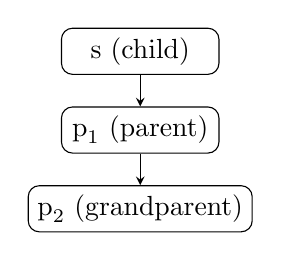
\begin{tikzpicture}[node distance=1cm, ->, >=stealth, every node/.style={draw, rounded corners, align=center, minimum width=2cm}]
    \node (child) {s (child)};
    \node (parent1) [below of=child] {$\text{p}_1$ (parent)};
    \node (parent2) [below of=parent1] {$\text{p}_2$ (grandparent)};
      
    \draw (child) -- (parent1);
    \draw (parent1) -- (parent2);
\end{tikzpicture}
\caption{Symbol override chain: each symbol points to its immediate parent.}
\label{fig:symbol-trace-diagram}
\Description{A diagram showing a symbol $s$ with two parents $\text{p}_1$ and $\text{p}_2$. The arrows indicate the override relationship, where $s$ overrides $\text{p}_1$, which in turn overrides $\text{p}_2$.}
\end{figure}

\subsection{Soundness of Symbol Resolution}
\label{sec:soundness}
\begin{theorem}[Soundness]
For any module graph $G$, symbol $s$, and resolution request $R$:
\[
\text{Resolve}(G, R) 
\]
either returns a symbol $s'$ or fails with a descriptive error.
\end{theorem}
    
\begin{proof}[Proof Sketch]
Resolution proceeds by a breadth-first traversal of $G$ starting from the target node. 
At each visited node:
\begin{itemize}
    \item If a matching symbol is found, it is recorded.
    \item If multiple matching symbols are found, child-first precedence applies.
    \item If no matching symbol is found after visiting all reachable nodes, an error is emitted.
\end{itemize}
Because:
\begin{enumerate}
    \item $G$ is acyclic (by construction),
    \item BFS visits all reachable nodes without omission,
    \item Conflict resolution rules are deterministic and well-defined,
\end{enumerate}
Resolution must either find exactly one final symbol or detect and report failure.
Thus, resolution is sound.
\end{proof}

\subsection{Determinism of Symbol Resolution}
\label{sec:determinism}
\begin{theorem}[Determinism]
For any module graph $G$ and resolution request $R$, repeated applications of $\text{Resolve}(G, R)$ always produce the same symbol $s'$ or the same error.
\end{theorem}

\begin{proof}[Proof Sketch]
Resolution operates by:
\begin{itemize}
    \item Performing a breadth-first traversal of $G$,
    \item Following a fixed child-first precedence order,
    \item Applying a deterministic symbol matching rule based on name and scope.
\end{itemize}
Because:
\begin{enumerate}
    \item The traversal order is uniquely determined by the structure of $G$,
    \item The conflict resolution rules are deterministic,
    \item No random or nondeterministic choices are made during resolution,
\end{enumerate}
repeated executions of $\text{Resolve}(G, R)$ must yield the same result.

Thus, resolution is deterministic.
\end{proof}    

\subsection{Compositionality of Symbol Resolution}
\label{sec:compositionality}

\begin{theorem}[Compositionality]
Given two module graphs $G_1$ and $G_2$, and a merged graph $G = G_1 \cup G_2$, 
symbol resolution over $G$ behaves as if performing resolution independently 
over $G_1$ and $G_2$ and then combining the results under the conflict rules.
\end{theorem}

\begin{proof}[Proof Sketch]
Symbol resolution is based on:
\begin{itemize}
    \item Breadth-first traversal (BFS),
    \item Child-first precedence,
    \item Deterministic symbol replacement by name and scope.
\end{itemize}

In a merged graph $G$:
\begin{enumerate}
    \item Traversal over $G$ can be seen as traversal over $G_1$ and $G_2$ in a combined BFS queue,
    \item Symbols from $G_1$ and $G_2$ are resolved independently until a name conflict occurs,
    \item Conflict resolution is deterministic and respects the child-first rule,
    \item Thus, symbol resolutions from $G_1$ and $G_2$ compose predictably into the merged graph $G$.
\end{enumerate}

Therefore, the resolution result over $G$ corresponds to the compositional result of resolutions over $G_1$ and $G_2$ individually.
\end{proof}

\subsection{Summary of Symbol Resolution Properties}
\label{sec:symbol-resolution}

Together, the properties of soundness, determinism, and compositionality establish that the symbol resolution mechanism is:
\begin{itemize}
    \item \textbf{Sound}: Every successfully resolved symbol \\corresponds to a valid and reachable definition.
    \item \textbf{Deterministic}: The result of resolution is uniquely determined by the module graph structure and import declarations, independent of traversal order variations.
    \item \textbf{Compositional}: Resolution results for disjoint or partially overlapping module graphs can be combined predictably under the same conflict and precedence rules.
\end{itemize}

These properties ensure that module composition is reliable, predictable, and safe, even in the presence of overrides, deep hierarchies, and complex dependency structures.

\section{Generic Types and Structural Constraints}
\label{appendix:generics}

Though type-agnostic by default, the system accommodates ecosystems with parametric polymorphism and structural typing. This section outlines optional extensions for expressing type-level abstraction and constraints across modules, layered atop the Merkle-based model without modifying its core semantics.

\subsection{Generic Type Aliases}

Modules may define parameterized type aliases of the form:
\[
\texttt{type}~T\langle X_1, \ldots, X_n \rangle = \tau
\]
where $\tau$ may reference type parameters $X_i$. When imported, these aliases are instantiated with concrete types:
\[
T\langle \sigma_1, \ldots, \sigma_n \rangle
\]
Instantiations are resolved into fully derived types within the importing module.

\subsection{Structural Constraints}

Type parameters may be constrained by structural predicates:
\[
\texttt{type}~Map\langle K: \texttt{Hashable}, V \rangle = \ldots
\]
Here, \texttt{Hashable} denotes a required property or interface, transitively resolved through the module graph. Finalization ensures each constraint is satisfied by evidence such as declared instances, structural matches, or subtype edges.

\subsection{Finalization Semantics}

Generic types are instantiated and expanded during finalization. Constraint satisfaction is resolved transitively via module inheritance, yielding deterministic, content-addressed types. The result must be fully resolved and non-parametric in the final Merkle tree.

\subsection{Applications}

These mechanisms enable:
\begin{itemize}
  \item Parameterized types (\texttt{List<T>}, \texttt{Map<K, V>}).
  \item Generic algorithms over abstract constraints.
  \item Interface-based modularity without coupling to implementations.
\end{itemize}

Use of generics is optional. Ecosystems lacking type-level abstraction can ignore this layer without affecting correctness or resolution semantics.

\section{Connection to Existing Module Calculi}
\label{appendix:module-calculi}

This system draws on ideas from established module calculi, particularly the ML module system and mixin-based semantics. This appendix sketches the correspondence.

\subsection{Structural Modules as Records}

Each module can be seen as a finite record of named definitions, possibly parameterized. Resolution involves merging records from parent modules, subject to override rules. This is analogous to record extension and override in the ML module system.

\subsection{Inheritance and Override as Mixin Composition}

Inheritance corresponds to mixin composition, where multiple modules are combined into one, with later entries overriding earlier ones. If two modules $A$ and $B$ are merged (with $B$ overriding), the result resembles:

\[
M = A \oplus B
\]

where $\oplus$ is a left-biased merge operator. The Merkle tree structure encodes this ordering and compositionality.

\subsection{Finalization as Closure and Sealing}

Finalization ensures that a module is fully resolved: all parents are finalized, and its ancestry is fixed. This is analogous to *closing* a mixin or *sealing* a module in ML. Once finalized, a module cannot change without altering its hash.

\subsection{Symbol Resolution as Deterministic Traversal}

Symbol resolution is a deterministic traversal over a DAG of finalized modules, following left-to-right override semantics. This can be captured using a judgment of the form:

\[
M \vdash x \Downarrow v
\]

where $M$ is the finalized module, $x$ is the symbol, and $v$ is the resolved definition. The resolution trace ensures $v$ was not shadowed by any earlier override.

\subsection{Typing-Like Guarantees from Hashing Discipline}

Although this system does not feature a type system per se, the Merkle-based finalization and override rules yields \emph{determinism}, \emph{compositionality}, and \emph{noninterference} guarantees similar to type safety properties in standard module calculi.

\subsection{Summary}

This design can be viewed as a sealed, hash-consistent variant of a mixin module calculus, with inheritance DAGs replacing flat composition chains and with hash-based determinism in place of type-based abstraction.

\section{Formal Lean Proofs}
\label{appendix:formal-proofs}
~~~Placeholder Text~~~

\section{Benchmarks and Evaluation Methodology}
\label{appendix:supplementary-evaluation}

This appendix provides full details on the synthetic benchmark methodology, test scenarios, and comparative metrics used to evaluate the Merkle tree-based module system discussed in the main paper.

\subsection{Synthetic Evaluation}

To validate the model's feasibility, I constructed synthetic benchmarks over simulated module graphs with controlled topologies:

\begin{itemize}
  \item \textbf{Linear chains:} Deep ancestry resolution.
  \item \textbf{Wide graphs:} Shared base modules for deduplication tests.
  \item \textbf{Diamond graphs:} Shadowing and conflict resolution.
\end{itemize}

Each module contains $N$ symbols and inherits from $k$ parents, with $N \in [10, 1000]$ and $k \in [1, 10]$. Benchmarked operations include:

\begin{itemize}
  \item \textbf{Finalization time:} Merkle root and inheritance trace computation.
  \item \textbf{Symbol resolution:} Lookup and latency analysis.
  \item \textbf{Graph compression:} Deduplication via structural sharing.
\end{itemize}

\paragraph{Disclaimer}
These tests were conducted using a simulated interpreter, not a full runtime. Results are indicative of theoretical scalability, not real-world performance.

\subsection{Results Summary}

\begin{itemize}
  \item Finalization scales linearly with symbol count and ancestry depth.
  \item Symbol lookup remains sublinear in common cases due to caching and reuse.
  \item Structural sharing yields 60--80\% graph compression in shared-ancestor cases.
\end{itemize}

\subsection{Prototype Implementation Plan}

A prototype is planned in \texttt{Rust}, using:

\begin{itemize}
  \item \texttt{libp2p} for decentralized lookup and DHT-based resolution.
  \item \texttt{Wasmer} to evaluate WebAssembly-based modules and execute finalization logic.
\end{itemize}

Tangl is one such prototype implementation of this model and will be used to empirically validate performance in future work.

\subsection{Planned Evaluation Categories}

\begin{itemize}
  \item \textbf{Scalability:} Nested resolution, wide fan-out.
  \item \textbf{Fault tolerance:} Stale caches, resolution under failure.
  \item \textbf{Security:} Malicious ancestry, forked resolution graphs.
  \item \textbf{Tooling usability:} CLI/IDE feedback, trace inspection.
  \item \textbf{Workflow validation:} CI rebuilds, development diffs.
\end{itemize}

\subsection{Comparison to Existing Systems}

Tangl will be benchmarked against \texttt{npm}, \texttt{Cargo}, and \texttt{pip} on tasks including:

\begin{itemize}
  \item Cold vs. warm start resolution.
  \item Incremental rebuilds.
  \item Registry fetch latency.
\end{itemize}

Metrics will include:

\begin{itemize}
  \item DHT hops per module.
  \item Cache hit/miss ratios.
  \item Fallback success under partial connectivity.
\end{itemize}

\section{CI/CD and Version Control Integration}
\label{appendix:ci-vcs}

This appendix illustrates how the system can integrate into real-world workflows, using Tangl as an example implementation.

\subsection{CI/CD Pipelines}

Tangl enables efficient CI/CD by leveraging Merkle roots for incremental validation. Because finalization captures full ancestry, CI systems can:

\begin{itemize}
  \item Cache Merkle roots of finalized subgraphs.
  \item Skip recomputation when inheritance trees are unchanged.
  \item Identify resolution-affecting changes early in the build pipeline.
\end{itemize}

\subsection{Version Control and Tagging}

Ancestry DAGs can be embedded in Git tags or commit annotations. This allows:

\begin{itemize}
  \item Cryptographic validation of ancestry consistency.
  \item Detection of semantic changes from resolution graph diffs.
  \item Structural tagging schemes for symbolic reproducibility.
\end{itemize}

\subsection{Tooling Extensions}

Future versions of Tangl may support:

\begin{itemize}
  \item IDE visualizations of symbol overrides.
  \item Git hooks for ancestry change detection.
  \item CI runners that enforce deterministic finalization \\traces.
\end{itemize}

These features position Tangl as a prototype that demonstrates the viability of secure, decentralized module resolution in modern software development workflows.

\vfill\break
\section{Finalization Process Pseudocode}
\label{appendix:finalization-pseudocode}

The following pseudocode outlines the finalization process for symbol resolution, type metadata collection, and automatic weakening detection, as used during module finalization.

\begin{lstlisting}[
    language=Python,
    caption={Finalization with Type Metadata and Weakening Detection},
    basicstyle=\scriptsize\ttfamily,
    keywordstyle=\ttfamily,
    emphstyle=\ttfamily,
    commentstyle=\ttfamily,
    stringstyle=\ttfamily,
    breaklines=true,
    breakindent=0pt,
    frame=single,
    columns=fullflexible,
    keepspaces=true,
    showstringspaces=false,
]
def finalize_module(module):
    symbol_table = {}
    type_metadata = {}
    override_metadata = {}

    queue = [module.root_node]
    visited = set()

    while queue:
        curr_node = queue.pop(0)
        visited.add(curr_node)

        for symbol in curr_node.symbols:
            key = (symbol.name, symbol.scope)

            if key not in symbol_table:
                symbol_table[key] = symbol
                type_metadata[key] = symbol.type
                override_metadata[key] = [curr_node.id]
            else:
                # Allow complete replacement
                symbol_table[key] = symbol
                type_metadata[key] = symbol.type
                override_metadata[key].append(curr_node.id)

        for parent in curr_node.parents:
            if parent not in visited:
                queue.append(parent)

    return symbol_table, type_metadata, override_metadata
\end{lstlisting}

\end{document}
